\section{Preliminary Work} \label{sec:preliminary-work}

We have a complete implementation of (1) the HPC 
We are actively porting this new algorithm to the cerebras software language, and have a prototype kernel already up and running with the Cerebras SDK at \url{https://github.com/mmore500/wse-sketches}.

\subsection{Asynchronous Agent-based Evolution Kernel}

\subsection{Hereditary Stratigraphy Implementation}

Existing work targets traditional HPC environments \citep{moreno2022hstrat}.
Although initial implementation of was designed in Python \citep{moreno2024hsurf}, we ported it (and its test suite) to CSL \citep{moreno2024wse}.

\subsection{Validation Experiment}

% fab w,h = 10,5
% Kernel x,y w,h = 4,1 3,3
% memcpy x,y w,h = 1,1 8,3
% whoami ===============================================================
% [[0 3 6]
%  [1 4 7]
%  [2 5 8]]
% whereami x ===========================================================
% [[0 1 2]
%  [0 1 2]
%  [0 1 2]]
% whereami y ===========================================================
% [[0 0 0]
%  [1 1 1]
%  [2 2 2]]
% cycle counter =======================================================
% [[120 120 120]
%  [120 120 120]
%  [120 120 120]]
% recv counter N ========================================================
% [[ 1  1  1]
%  [33 31 29]
%  [29 28 29]]
% recv counter S ========================================================
% [[31 33 31]
%  [33 31 29]
%  [ 1  1  1]]
% recv counter E ========================================================
% [[31 29  1]
%  [28 29  1]
%  [30 33  1]]
% recv counter W ========================================================
% [[ 1 28 29]
%  [ 1 31 32]
%  [ 1 33 30]]
% send counter N ========================================================
% [[  0   0   0]
%  [124 130 124]
%  [132 122 114]]
% send counter S ========================================================
% [[130 126 112]
%  [118 112 118]
%  [  0   0   0]]
% send counter E ========================================================
% [[112 116   0]
%  [124 130   0]
%  [132 122   0]]
% send counter W ========================================================
% [[  0 126 112]
%  [  0 112 118]
%  [  0 120 128]]

In addition to unit and integration tests, we performed an experiment to validate reconstructions performed.
Due to the limitations of the hardware simulator, we performed this experiment using a 3x3 grid of processor elements.
We ran for 120 generations with a population size of 32 per PE, and a tournament size of 5.
Genomes were fixed-length 3 word arrays represented using data type \texttt{u32}.
The send buffer was configured to hold one genome and the receive buffers held 3 genomes.
between 28 and 33 receive cycles completed for each PE.
Between 112 and 132 send cycles completed for each PE.

v0.1.0 of the wse-sketches repository \citep{moreno2024wse} and v1.0.0 of the cerebras SDK \citep{selig2022cerebras}.

\begin{figure}[htbp]
    \centering

    % Top panel for the image
    \begin{subfigure}[b]{\textwidth}
        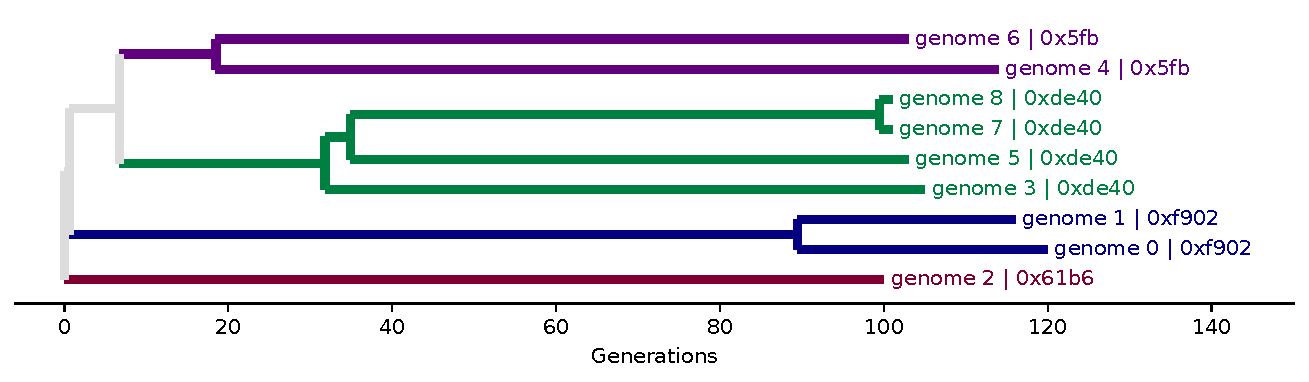
\includegraphics[width=\textwidth]{binder/binder/teeplots/genome=hsurftiltedsticky_tagged+viz=draw-biopython-tree+ext=}
        \caption{Caption for the image}
    \end{subfigure}

    % Space between image and table
    \vspace{10pt} 

    % Bottom panel for the table
    \begin{subfigure}[b]{\textwidth}
        \centering
    \begin{tabular}{
    c
    >{\columncolor{LighterBlue}}c
    >{\columncolor{LighterBlue}}c
    >{\columncolor{LighterSalmon}}c
    >{\columncolor{LighterSalmon}}c
    q % Thick divider
    >{\columncolor{LighterPastelGreenYellow}}c
    >{\columncolor{LighterPastelGreenYellow}}c
    >{\columncolor{LighterPastelGreenYellow}}c
    >{\columncolor{LighterPastelGreenYellow}}c
    q % Thick divider
    >{\columncolor{LighterPastelGreenYellow}}c
    >{\columncolor{LighterPastelGreenYellow}}c
    >{\columncolor{LighterPastelGreenYellow}}c
    >{\columncolor{LighterPastelGreenYellow}}c
    }
    & \multicolumn{4}{cq}{\cellcolor{white}Word 0} & \multicolumn{4}{cq}{\cellcolor{white}Word 1} & \multicolumn{4}{c}{\cellcolor{white}Word 2} \\
    \cmidrule(l{1.5pt}r{1.5pt}){2-5}
    \cmidrule(l{1.5pt}r{1.5pt}){6-9}
    \cmidrule(l{1.5pt}r{1.5pt}){10-13}
    & {\cellcolor{white}B 0} & {\cellcolor{white}B 1} & {\cellcolor{white}B 2} & {\cellcolor{white}B 3} & {\cellcolor{white}B 4} & {\cellcolor{white}B 5} & {\cellcolor{white}B 6} & {\cellcolor{white}B 7} & {\cellcolor{white}B 8} & {\cellcolor{white}B 9} & {\cellcolor{white}B 1}0 & {\cellcolor{white}B 1}1 \\
    \cmidrule(l{1.5pt}r{1.5pt}){2-2}
    \cmidrule(l{1.5pt}r{1.5pt}){3-3}
    \cmidrule(l{1.5pt}r{1.5pt}){4-4}
    \cmidrule(l{1.5pt}r{1.5pt}){5-5}
    \cmidrule(l{1.5pt}r{1.5pt}){6-6}
    \cmidrule(l{1.5pt}r{1.5pt}){7-7}
    \cmidrule(l{1.5pt}r{1.5pt}){8-8}
    \cmidrule(l{1.5pt}r{1.5pt}){9-9}
    \cmidrule(l{1.5pt}r{1.5pt}){10-10}
    \cmidrule(l{1.5pt}r{1.5pt}){11-11}
    \cmidrule(l{1.5pt}r{1.5pt}){12-12}
    \cmidrule(l{1.5pt}r{1.5pt}){13-13}
    & \multicolumn{4}{cq}{\cellcolor{white}} & \multicolumn{4}{cq}{\cellcolor{white}} & \multicolumn{4}{c}{\cellcolor{white}} \\[-2ex]
    Genome 1 & \texttt{F9} & \texttt{02} & \texttt{79} & \texttt{00} & \texttt{8D} & \texttt{22} & \texttt{4F} & \texttt{F3} & \texttt{D2} & \texttt{78} & \texttt{AD} & \texttt{C7} \\
    & \multicolumn{4}{cq}{\cellcolor{white}} & \multicolumn{4}{cq}{\cellcolor{white}} & \multicolumn{4}{c}{\cellcolor{white}} \\[-2ex]
    Genome 2 & \texttt{F9} & \texttt{02} & \texttt{75} & \texttt{00} & \texttt{8D} & \texttt{A1} & \texttt{CB} & \texttt{F2} & \texttt{D1} & \texttt{5B} & \texttt{CC} & \texttt{D4} \\
    & \multicolumn{4}{cq}{\cellcolor{white}} & \multicolumn{4}{cq}{\cellcolor{white}} & \multicolumn{4}{c}{\cellcolor{white}} \\[-2ex]
    Genome 3 & \texttt{61} & \texttt{B6} & \texttt{65} & \texttt{00} & \texttt{66} & \texttt{29} & \texttt{B4} & \texttt{F0} & \texttt{62} & \texttt{99} & \texttt{5A} & \texttt{61} \\
    {\cellcolor{white}\ldots} & {\cellcolor{white}\ldots} & {\cellcolor{white}\ldots} & {\cellcolor{white}\ldots} & {\cellcolor{white}\ldots} & {\cellcolor{white}\ldots} & {\cellcolor{white}\ldots} & {\cellcolor{white}\ldots} & {\cellcolor{white}\ldots} & {\cellcolor{white}\ldots} & {\cellcolor{white}\ldots} & {\cellcolor{white}\ldots} \\
    \end{tabular}

        \caption{Caption for the table}
    \end{subfigure}

    \caption{Caption for the entire figure}
    \label{fig:my_figure}
\end{figure}



    % \begin{tabular}{
    % c
    % >{\columncolor{LighterBlue}}c
    % >{\columncolor{LighterBlue}}c
    % >{\columncolor{LighterSalmon}}c
    % >{\columncolor{LighterSalmon}}c
    % q % Thick divider
    % >{\columncolor{LighterPastelGreenYellow}}c
    % >{\columncolor{LighterPastelGreenYellow}}c
    % >{\columncolor{LighterPastelGreenYellow}}c
    % >{\columncolor{LighterPastelGreenYellow}}c
    % q % Thick divider
    % >{\columncolor{LighterPastelGreenYellow}}c
    % >{\columncolor{LighterPastelGreenYellow}}c
    % >{\columncolor{LighterPastelGreenYellow}}c
    % >{\columncolor{LighterPastelGreenYellow}}c
    % }
    % & \multicolumn{4}{cq}{\cellcolor{white}Word 0} & \multicolumn{4}{cq}{\cellcolor{white}Word 1} & \multicolumn{4}{c}{\cellcolor{white}Word 2} \\
    % \cmidrule(l{1.5pt}r{1.5pt}){2-5}
    % \cmidrule(l{1.5pt}r{1.5pt}){6-9}
    % \cmidrule(l{1.5pt}r{1.5pt}){10-13}
    % & {\cellcolor{white}B 0} & {\cellcolor{white}B 1} & {\cellcolor{white}B 2} & {\cellcolor{white}B 3} & {\cellcolor{white}B 4} & {\cellcolor{white}B 5} & {\cellcolor{white}B 6} & {\cellcolor{white}B 7} & {\cellcolor{white}B 8} & {\cellcolor{white}B 9} & {\cellcolor{white}B 1}0 & {\cellcolor{white}B 1}1 \\
    % \cmidrule(l{1.5pt}r{1.5pt}){2-2}
    % \cmidrule(l{1.5pt}r{1.5pt}){3-3}
    % \cmidrule(l{1.5pt}r{1.5pt}){4-4}
    % \cmidrule(l{1.5pt}r{1.5pt}){5-5}
    % \cmidrule(l{1.5pt}r{1.5pt}){6-6}
    % \cmidrule(l{1.5pt}r{1.5pt}){7-7}
    % \cmidrule(l{1.5pt}r{1.5pt}){8-8}
    % \cmidrule(l{1.5pt}r{1.5pt}){9-9}
    % \cmidrule(l{1.5pt}r{1.5pt}){10-10}
    % \cmidrule(l{1.5pt}r{1.5pt}){11-11}
    % \cmidrule(l{1.5pt}r{1.5pt}){12-12}
    % \cmidrule(l{1.5pt}r{1.5pt}){13-13}
    % & \multicolumn{4}{cq}{\cellcolor{white}} & \multicolumn{4}{cq}{\cellcolor{white}} & \multicolumn{4}{c}{\cellcolor{white}} \\[-2ex]
    % Genome 1 & \texttt{F9} & \texttt{02} & \texttt{79} & \texttt{00} & \texttt{8D} & \texttt{22} & \texttt{4F} & \texttt{F3} & \texttt{D2} & \texttt{78} & \texttt{AD} & \texttt{C7} \\
    % & \multicolumn{4}{cq}{\cellcolor{white}} & \multicolumn{4}{cq}{\cellcolor{white}} & \multicolumn{4}{c}{\cellcolor{white}} \\[-2ex]
    % Genome 2 & \texttt{F9} & \texttt{02} & \texttt{75} & \texttt{00} & \texttt{8D} & \texttt{A1} & \texttt{CB} & \texttt{F2} & \texttt{D1} & \texttt{5B} & \texttt{CC} & \texttt{D4} \\
    % & \multicolumn{4}{cq}{\cellcolor{white}} & \multicolumn{4}{cq}{\cellcolor{white}} & \multicolumn{4}{c}{\cellcolor{white}} \\[-2ex]
    % Genome 3 & \texttt{61} & \texttt{B6} & \texttt{65} & \texttt{00} & \texttt{66} & \texttt{29} & \texttt{B4} & \texttt{F0} & \texttt{62} & \texttt{99} & \texttt{5A} & \texttt{61} \\
    % {\cellcolor{white}\ldots} & {\cellcolor{white}\ldots} & {\cellcolor{white}\ldots} & {\cellcolor{white}\ldots} & {\cellcolor{white}\ldots} & {\cellcolor{white}\ldots} & {\cellcolor{white}\ldots} & {\cellcolor{white}\ldots} & {\cellcolor{white}\ldots} & {\cellcolor{white}\ldots} & {\cellcolor{white}\ldots} & {\cellcolor{white}\ldots} \\
    % \end{tabular}



Data from this experiment is available via the Open Science Framework at \url{https://osf.io/bfm2z/} \citep{moreno2024toward}.
